\chapter{Analysis of the hardware}
Based on the conclusions from the previous chapter, it is now possible to decide what features are expected from the controllers and what is their importance.

\section{Prioritization of the features}
The chosen device is expected to have a defined set of features - but not all of them have equal priority. MoSCoW analysis will be used to determine which features are most important\cite{moscow}. It is usually used in deciding on priorities of requirements with stakeholders, but can be applied to any requirements-related problem. It segregates features in four different groups: \begin{itemize}
\item \emph{must have} - features, that are critical for success of the project
\item \emph{should have} - features, that are usually as important as critical, but not having them won't fail the project
\item \emph{could have} - features, that are desirable and usually can be easily obtained 
\item \emph{would like, but won't get} - features that are least critical and not in any way decisive 
\end{itemize}

Now it is possible to group the requirements acquired from previous chapter as following:
\begin{itemize}
\item Must have
\begin{itemize}
\item detailed gesture recognition supported out-of-the-box
\item price not bigger than 300\$
\item acceptable documentation and any kind of support for Unity
\item high comfort of usage in means of wearing/handling and range
\item be available for customer use
\item excellent precision
\end{itemize}
\item Should have
\begin{itemize}
\item excellent documentation
\item support for Unity provided by the manufacturer
\item worldwide availability 
\item community significant in size
\item acceptable precision
\end{itemize}
\item Could have
\begin{itemize}
\item physical feedback
\item price lower than 200\$
\end{itemize}
\item Won't have
\end{itemize}


\section{Devices}
%write about why you have chosen those devices and not other
The devices for evaluation where picked based on their accessibility for testing. Devices listed above are all available for commercial use and have prices lower than 300\$ per piece. Following devices will be evaluated:


\subsection[title=Wii Remote]{Wii Remote - based on \cite{wiiu, wii_spec, wii_article}}

\begin{wrapfigure}{l}{0.5\textwidth}
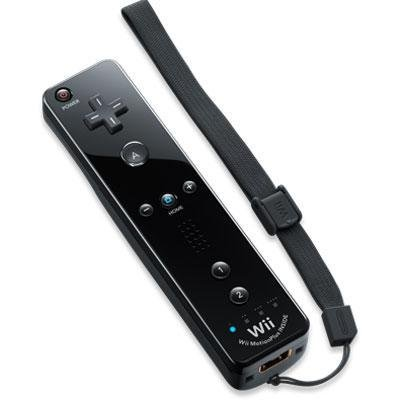
\includegraphics[width=0.48\textwidth]{graphics/wiiremote.jpg} 
\caption{Wii Remote by Nintendo}
\vspace{-10pt}
\label{fig:wii}
\end{wrapfigure}

The Wii Remote (Wiimote) device is absolute pioneer in the motion tracking for gaming. It was released in 2006 by Nintendo for their new Wii Console, but the concept was invented as early as in 2001 by a company commissioned by Nintendo. 

The important part of Wii Remote set in Sensor Bar, containing ten infrared LEDs, five next to each end, with the outermost lights pointing a little bit more to the outside, and the inner ones - to the inside. The Wiimote acts like a remote controller, as the motion detection requires the controller to point at Sensor Bar. The Wii Remote contains optical sensor, that using the position of two source of lights (left and right edge) is able to calculate the distance and position and send it to console via Bluetooth. The device optimal range is up to 5 meters from the Sensor Bar. It also includes accelerometer, as well as rumble and audio feedback. The later versions (Wii Remote Plus, to which Wii Remote can be upgraded) also contains gyroscope. The controller has eight buttons and control pad. Important part of the design is also a wrist strap, allowing to lock the device on a hand, stopping from accidental throwing during quick, energetic movements. Because of the design, it does not offer gesture recognition.

The documentation and SDK is available upon registration and acceptance from the Nintendo, so it was not possible to estimate the quality of it. There is no official plugin for Unity from Nintendo and those delivered by community are of poor quality. 

The device is available worldwide by both online and stationary shops.

\subsection[title=Play Station Move]{PlayStation Move - based on \cite{psmove, psmove_spec}}

\begin{wrapfigure}{r}{0.5\textwidth}
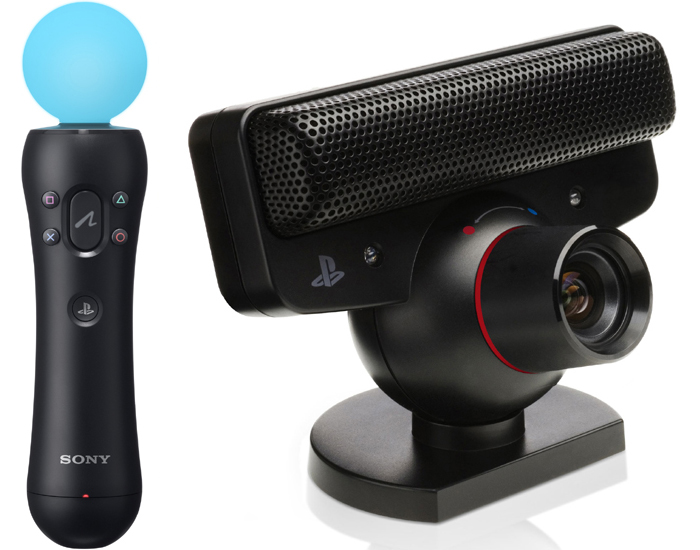
\includegraphics[width=0.48\textwidth]{graphics/move.jpg} 
\caption{Play Station Move (left) and Play Station Eye (right) by Sony Computer Entertainment}
\vspace{-10pt}
\label{fig:move}
\end{wrapfigure}

PlayStation Move (with its important component, PlayStation Eye or PlayStation Camera) is a product of Sony Computer Entertainment and was designed for the PlayStation 3 as an answer to Nintendo Wii Remote in 2009. Similar in look, as can be seen in figure \ref{fig:move}, PlayStation Move is a wand-like controller communicating through a Bluetooth 2.0, but the most important part of its design is an orb on the top of it, able to light up in different colors. The color is picked by the software to provide best distinction from the rest of scene. Known size of light allows the camera to precisely evaluate the distance and provide the position in all three dimensions. The simple sphere shape-based calculation allows high precision and accuracy. 

PlayStation Move also contains  accelerometer, gyroscope and even terrestrial magnetic field sensor to correct against drift caused by inertial sensors. Internal temperature sensor was also used in order to correct other sensor readings based on temperature effects. The sensors allows to estimate players position even if the orb is not visible to camera at the moment. The wand also has 8 buttons. It provides vibration feedback and visual one - from the orb.

Sony offers acceptable documentation and explicit support for Unity. However, obviously they do not provide any gesture recognition. The developer has access to buttons, position data and raw data. 

The price is very low, while the product is available worldwide, also in stationary shops.

\begin{wrapfigure}{l}{0.5\textwidth}
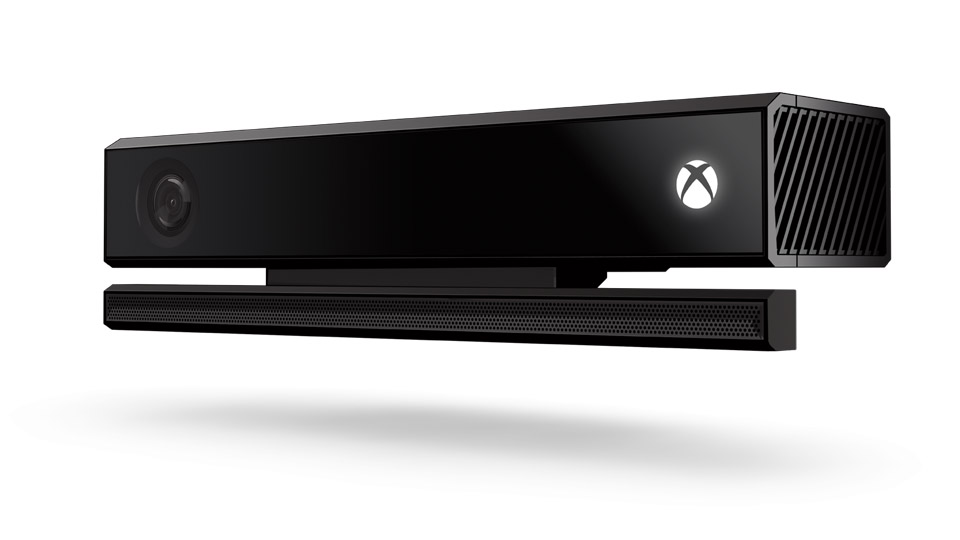
\includegraphics[width=0.48\textwidth]{graphics/kinect.jpg} 
\caption{Microsoft Kinect for XBox One}
\vspace{-10pt}
\label{fig:kinect}
\end{wrapfigure}

\subsection{Microsoft Kinect - based on \cite{Kinect,kinect_spec,handpose}}

The Microsoft Kinect is a series of motion tracking products for Microsoft Xbox consoles. The first Kinect was released in 2010, and two years later its second version for Xbox One entered the market.

The device uses significantly different technology than its main competitors - Wii Remote and PlayStation Move. As shown in figure \ref{fig:kinect}, Kinect do not have any controllers - it's camera based solution, where motion tracking is fully performed by only processing the image of a moving person, who does wear any type of calibration devices. The laters Kinect sensor contains 1080p camera, infrared emitter, infrared depth sensor, accelerometer and microphones array. Those features allows motion recognition in a range 0.5 to 4.5 meters from the Kinect with 4-centimetre cube precision and voice recognition. The sensor detects movement of the whole body with recognizing up to 20 joints.

Microsoft Kinect has an excellent documentation, explicit support for Unity and SDKs for C++, C\# and Visual Basic .Net. It has an acceptable price and is available worldwide in both online and stationary shops.
 
As for now, Microsoft Kinect do not provide gesture recognition, but there are promising official demos showing the software upgrade providing such features. Unfortunately, it is not expected to enter the market for the next few years.

\subsection{Creative Senz3D - based on \cite{senz_parts, senz, senz_opencv}}

\begin{wrapfigure}{r}{0.5\textwidth}
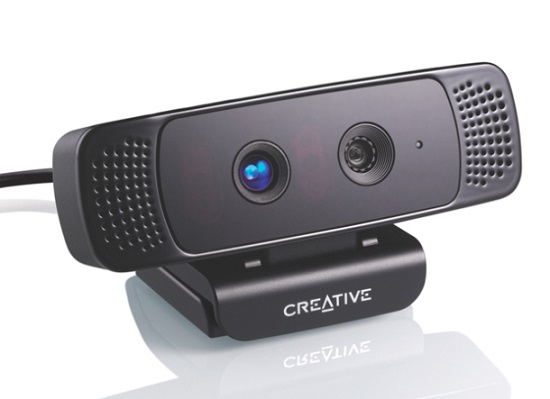
\includegraphics[width=0.48\textwidth]{graphics/senz.jpg} 
\caption{Creative Senz3D}
\vspace{-8pt}
\label{fig:senz}
\end{wrapfigure}

Creative Senz3D is a product released by Creative Technologies Ltd. in 2013. It is the predecessor of Intel RealSense camera and as though, is not longer actively supported. 

Senz3D contains laser for scene illumination, depth sensor for gesture recognition, HD camera for video capturing and dual array microphones. It allows detecting hand and head gestures as well as face recognition and to some extent also voice recognition. The preferred range is 20 to 50 cm.

Because the project is discontinued, it is extremely hard to obtain the SDK via official ways. It means that there is also no actual documentation. There is no support for Unity, but the OpenCV library, popular solution for image recognitions, has a wrapper for it.

Device has an acceptable price and is available through few online sellers. 

\subsection{Myo - based on \cite{myo, myo_specs, myo_article}}

\begin{wrapfigure}{r}{0.5\textwidth}
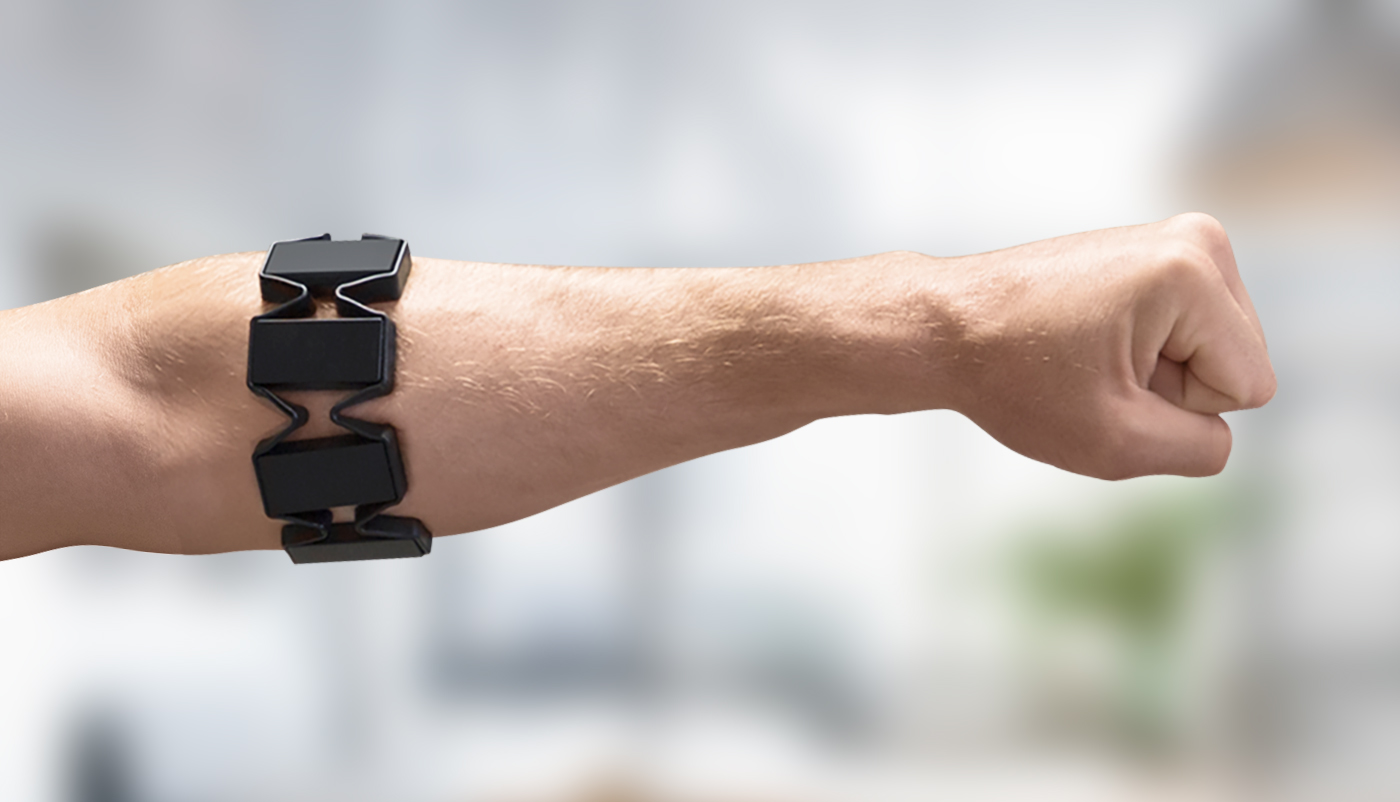
\includegraphics[width=0.48\textwidth]{graphics/myo.jpg} 
\vspace{-8pt}
\caption{Myo armband by Thalmic Labs}
\label{fig:myo}
\end{wrapfigure}

Myo is an armband, released by Thalmic Labs at the beginning of 2015, with developer access starting in 2014. It achieves detailed gesture recognition using unique technology in this industry, which is detecting the electrical impulses sent to the muscles (electromyography - EMG). 

The device contains 8 EMG sensors, accelerometer, gyroscope, magnetometer and provides feedback with vibration. It communicates with computer through Bluetooth 4.0 LE. 

It has excellent documentation and explicit Unity support. It offers not only raw data from the sensors, but is also able to detect five unique gestures, like fist, waving or tapping. It has a little higher than average price and is available worldwide by shimpent and in some shops in North America. 



\subsection[title=Leap Motion]{Leap Motion - based on \cite{Leap, leap_article, leap_pop}}

\begin{wrapfigure}{l}{0.5\textwidth}
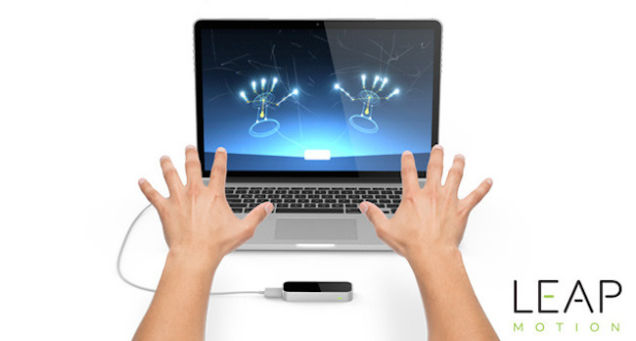
\includegraphics[width=0.48\textwidth]{graphics/leap.jpg} 
\caption{Leap Motion by Leap Motion Inc}
\vspace{-9pt}
\label{fig:leap}
\end{wrapfigure}

Leap Motion is a camera-based device dedicated to hand, or rather palm movement tracking. Although the idea behind the technology was first developed in 2008, the product was released to developers in 2012 and entered the market in 2013. However, the device did not sell as well as expected. In 2014 the company released second version of software for developers and started combining its product with VR, which is the main commercial usage up to day.

The device is a small box, as shown in fig. \ref{fig:leap}. It contains two infrared cameras and three infrared LEDs. The field of view is a hemisphere, with range up to 1 m. 

Leap Motion has an excellent documentation and a significant developers community, involved in many projects, also medical ones. It has an explicit support for Unity and SDK supporting most of popular modern languages (JS, C\#, C++, Java, Python, Objective-C). The support for Unity also includes examples of how to connect it with Oculus Rift. The data send through SDK is the position of detected joints, but also detection of simple gestures like tapping, swiping.

The device has a low price and is available worldwide, not only with shipment from the producer, but also in stationary and online shops across four continents. 


\subsection{Sphero 2.0 - based on \cite{sphero, sphero_review}}

\begin{wrapfigure}{r}{0.5\textwidth}
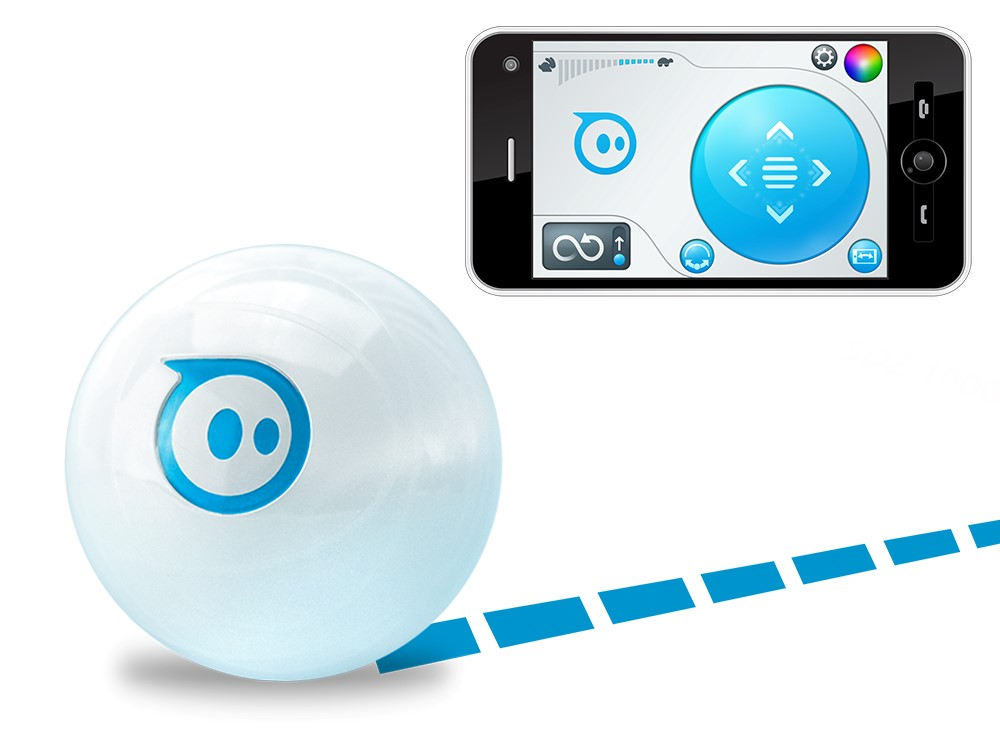
\includegraphics[width=0.48\textwidth]{graphics/sphero.jpg} 
\vspace{-8pt}
\caption{Sphero 2.0 by Sphero}
\label{fig:sphero}
\end{wrapfigure}

The Sphero is a spherical robot toy, which prototype was first shown in 2010. The version 2.0 was released in 2013 by Orbotix (now Sphero). The device is a sealed ball, containing gyroscope, accelerometer, electric motor allowing  speed to up 7.3 km/h, LEDs and and polycarbonate shell. 

Sphero is controlled with app through Bluetooth. The App allows moving the ball around, changing its color and shaking it. Sphero can be used as a motion detector using the gyroscope and accelerometer.

It can be used with any device that can connect to it through Bluetooth. It has excellent documentation and support for Unity, however only for mobiles. It has an average price and is available worldwide through online shopping. It does not offer gesture recognition.

\section{Evaluation}

The evaluation will have following criteria, grouped from MoSCoW analysis:
\begin{itemize}
\item Critical requirements:
\begin{itemize}
	\item precision: high/average/bad
	\item range: good/bad/not applicable
	\item gesture recognition: have/do not have
\end{itemize}
\item Important requirements:
\begin{itemize}
	\item price: low (<75\$), average (75-150\$), high (>150\$) 
	\item documentation: good, average, bad, available upon registration
	\item support for Unity: have, have partial, do not have
	\item availability: great (both online and stationary shops around the world), good (worldwide shipment and some stationy shops), average (worldwide shipment), bad (shipment to only few countries).
	\item community: good (>1000 question on Stack Overflow and own Dev Forum), average (1000-500 questions on Stack Overflow and own Dev Forum), bad (<500 questions on Stack Overflow or own Dev Forum).
\end{itemize}
\item Useful features:
\begin{itemize}
	\item feedback: have/do not have
\end{itemize}
\end{itemize}

The summary of the analysis is described in tables \ref{tab:hardware} and \ref{tab:hardware2}.

\subsection{Comments}
Although most of the criteria has been explained in previous section, some of the experimentally evaluated ones needs further explanations.
\subsubsection{Precision}
Precision was evaluated by testing all of the devices and observing to factors - delay and accuracy of movement. The reason, why Senz3D, Leap Motion and Sphero 2.0 has average grade is that the former has too high detection rate and cannot always detect hands and the latter have low accuracy.
\subsubsection{Range}
The Leap Motion is the only device who received "bad" range evaluation. It is caused by the fact, that while playing with the device it is easy to, instead of reaching for an object, remove the hand from the device's field of view. The FOV is small and except for small gestures, no broader movements cannot be made.

\section{Conclusions}
The devices PS Move and Myo have similar, very high number of positively evaluated factors. The final choice for the device will be Myo, because built-in gesture recognition have higher priority than price lower than 200\$. 

\begin{table}[t]
\centering
\caption{The summary of analysis of the devices, part 1}
\label{tab:hardware}
\begin{tabular}{|c|c|c|c|c|c|c|c|}
 \hline
  Criterion:          & Wii Remote          	& PS Move     		& Microsoft Kinect \\
  \hline 
  precision           & \greentick high      	& \greentick high   & \greentick high  \\
  \hline
  range               & \greentick good      	& \greentick good	& \greentick good \\
  \hline
  gesture recognition & \redcross don't have 	& \redcross don't have  & \redcross don't have  \\
  \hline
  price               & \greentick  low          & \greentick  low     & \yellowdmd average     \\
  \hline
  documentation       & \yellowdmd after registration  	& \yellowdmd average & \greentick good \\
  \hline
  support for Unity   & \redcross don't have    & \greentick have    & \greentick have \\ 
  \hline
  availability        & \greentick great        & \greentick great   & \greentick great\\   
  \hline
  community           & \yellowdmd average     	& \greentick good     & \greentick good\\    
  \hline
  feedback            & \greentick vibration \& audio  & \greentick vibration   & \redcross none \\       
  \hline
\end{tabular}
\end{table}

\begin{table}[t]
\centering
\caption{The summary of analysis of the devices, part 2}
\label{tab:hardware2}
\begin{tabular}{|c|c|c|c|c|c|c|c|}
  \hline
  Criterion:           & Senz3D     		   	& Myo       		   & Leap Motion 		& Sphero 2.0 \\
  \hline 
  precision            & \yellowdmd average    	& \greentick high      & \yellowdmd average & \yellowdmd average\\
  \hline
  range                & \greentick good       	& N/A       		   & \redcross bad      & \greentick good \\
  \hline
  gesture recognition  & \redcross don't have 	& \greentick have      & \greentick have    & \redcross don't have  \\
  \hline
  price                & \redcross high       	& \redcross high 	   & \yellowdmd average & \yellowdmd average\\
  \hline
  documentation        & \redcross bad        	& \greentick good      & \greentick good    & \greentick good \\
  \hline
  support for Unity    & \redcross don't have 	& \greentick have      & \greentick have    & \yellowdmd have partial \\
  \hline
  availability         & \yellowdmd average    	& \greentick good      & \greentick great   &\greentick  good\\
  \hline
  community            & \redcross bad        	& \yellowdmd average   & \yellowdmd average & \redcross bad \\
  \hline
  feedback             & \redcross none       	& \greentick vibration & \redcross none     & \greentick vibration \& light \\
  \hline
\end{tabular} 
\end{table}